\chapter{Marco Teórico}
\label{ch:Marco Teórico}

Es importante introducir al lector en los conceptos principales que forman parte del análisis de componentes principales, dentro del cual se hará énfasis con un enfoque estadístico dentro del mismo. En este capítulo, se dará una introducción al del análisis de componentes principales para conocer su evolución; así como los enfoques que existen dentro del mismo. Posteriormente, se explicarán temas el cálculo de componentes y la interpretación de ellos.

\section{¿Qué es el análisis de componentes principales?}

El análisis de componentes principales o por sus siglas en ingles PCA (Principal Components Analysis) es una estrategia de reducción de datos usada usualmente con tres enfoques matemáticos y estadísticos los cuales son:  

\begin{itemize}
    \item \textbf{Enfoque descriptivo} tiene como objetivo principal el uso de matemática aplicada. Se proyecta por medio una recta los diferentes puntos, lo cual se desea que estos se mantenga en cercanía a la recta. En la figura \ref{fig:rectaPCA} podemos observar un ejemplo gráfico de lo explicado anteriormente.   
    \item \textbf{Enfoque estadístico} el autor Andrés Sánchez nos explica que este enfoque busca minimizar la dimensión de un conjunto con gran cantidad de variables. A partir de una proyección de los datos se alcanzará una nueva representación con los componentes con menor varianza. \footnote{La varianza mide el nivel de dispersión de los valores de las variable con respecto a la media  aritmética[Fuente: \href{https://cutt.ly/FmJ69v4}{https://cutt.ly/FmJ69v4}]} Este enfoque se verá a mayor profundidad en la sección \ref{Enfoque estadístico}. \cite{andresSanchesMangas}
    \item \textbf{Enfoque geométrico} implementa una serié de representaciones gráficas por las cuales se ilustran la proyección de datos resultante, por medio de rectas en un plano en los que se incluyen los puntos, ya sea de forma 2D y/o 3D en la figura \ref{fig:representacionPCA} y \ref{fig:representacion3D} podrá observar ejemplos de representación. 
\end{itemize}

En cuanto al objetivo principal es la extracción de una serie de datos, sin que se penalice la perdida considerable de variables. El planteamiento del PCA es que posee valores de variables que se denominan \textbf{p-variables} en un número de elementos llamados \textbf{n-elementos} con los que se cuenta en una población determinada. Estos p-variables y n-elementos se posicionan en una matriz \textit{X} de tamaño \textit{n x p}, donde \textbf{p-variables} son las columnas de la matriz y \textbf{n-elementos} son las filas. 

$$ X = \begin{pmatrix} p-variables_{11} &  p-variables_{12}  &     \cdots   &    p-variables_{1n}\\
                      n-elementos_{21} &  n-elementos_{22}  &   \cdots  &    n-elementos_{2n} \\
                        \vdots    &  \vdots  &   \ddots  & \vdots  \\
                        n-elementos_{nx1}    &  n-elementos_{nx2}   & \cdots &   n-elementos_{nxn}
       \end{pmatrix}$$

Como se explicó con anterioridad el objetivo principal es reducir la dimensión del conjunto de datos de entrada a costo de una mínima perdida de información. Donde el resultado de reducir el conjunto de variables, es menor que las p-variables originales es decir, \textbf{r > p}. 

\notebox{
Para explicar de una forma más clara la reducción de dimensiones. Consiste en tablas de \textit{n} columnas, las cuales se le aplica la reducción, convirtiendo esta tabla de \textit{n} columnas en \textit{n - x}. Por ejemplo: Contamos con 5 columnas, al realizar esta técnica de reducción, tendremos como resultado 2 columnas los cuales estas dos columnas capturan la mayor información de la tabla original. 
}

 
 \section{¿Cómo surge el PCA?}
El origen es difícil de establecer, por lo que derivan independientemente las expresiones de la descomposición en valores singular en la forma utilizada por el PCA. Así mismo, se adoptaron diferentes aproximaciones, como mejorar contrar lineas y planos que mejoren le conjunto de datos en un espacio, donde optimizaran los problemas hacia los que se dirigían las componentes principales \cite{andresSanchesMangas}

Pearson, como nos lo menciona Sánchez, comenta que de acuerdo con la computación, sus métodos podrían tener una resolución más factible a los problemas númericos.
En un principio, los cuatro trabajos más importantes según Sánchez:

El primero, escrito por Anderson, el más teórico. El cuál "dicute el muestreo de distribuciones asintóticas de coeficientes y virianzas de muestras de componentes principales." \cite{andresSanchesMangas}

El segundo, por Rao. Donde "resalta por el grán número de nuevas ideas concernientes al uso, interpretación y extension del PCA que se introducen." \cite{andresSanchesMangas}

En tercer lugar, dado por Gower, que discute uniones y otras técnicas del PCA.

Y en cuarto lugar, con un gran ímpetu, Jeffers da al "lado práctico den este campo mediante la comparación de dos casos de estudio"\cite{andresSanchesMangas} que con el PCA se trata de llegar más lejos de la reducción de dimensiones.

Cabe recalcar que el PCA, al no tener en cuenta el objetivo de los datos, abre una puerta al uso, facilidad y versatilidad de muchas aplicaciones.


\section{Cálculo de componentes}

Dentro del PCA hay maneras de calcular los componentes principales, siguiendo como guía las menciones de \cite{rojas2009analisis}, que aborda de manera clara la manera de realizarlos.

\subsection{En el espacio del individuo}

Se debe suponer que ya las variables se encuentran centradas y reducidas, Donde $V=\dfrac{1}{n}X^t X$ es la matriz de varianzas-covarianza, así que como las variables están reducidas y centradas entonces $V=R$, siendo la matriz de correlación:

$$ u_{ij}=cov(X^i , X^j)=\dfrac{cov(X^i , X^j)}{\sigma X^i \sigma X^j}=R(X^i , X^j)$$

De esta manera el espacio de las filas de $X$ en $\mathbb{R}^m$ es el espacio de individuos cuyo origen será el centro del conjunto de puntos, teniendo como objetivo describir de manera simétrica el conjunto de datos mediante el PCA.

\subsection{Teorema 1}

En la primera etapa de un PCA se debe calcular el eje $D_1$ que paso por el origen para la cual el conjunto de puntos sea máximo, así este eje $D_1$ pasa lo más cerca del conjunto de datos, queriendo decir que el promedio de las distancias al cuadrado de los $n$ puntos del conjunto y el eje $D_1$ es minimal.

Sea $a^1$  vector director normado del eje $D_1$ \textbf{entonces: } $a^1$ es el vector propio asociado al valor propio más grande de la matriz $V$ de varianzas-covarianzas.

Pero mucho antes de probar el teorema se necesita del la siguiente proposición que deberá ser tomada como válida.

\notebox{
Sean $A$ y $B$ dos matrices cuadradas $m$ x $m$ simétricas y sea $A$ una matriz definida positiva, de esta manera el vector $y$ $\in$ $\mathbb{R}^n$ que puede resolver la siguiente optimización:
\[\left\{ \begin{array}{rcl}
\mbox{max } y^t By \\
& & \\
\mbox{sujeto a } y^t Ay=1 \\
\end{array}
\right. \]

es el vector propio de $a^1$ de $A^{-1}B$ de norma 1 asociado al valor mas grande $\beta_1$.

}

Las coordenadas de los valores $i$-ésimo son:
 
 $$i=(x_{i1},...,x_{ij},...,x_{im})$$
 
 Además se sabe que la proyección del valor $i$ sobre le eje $D_1$ es:
 
 
 $$P(i,D_1)=\dfrac{\langle i, a^1 \rangle}{||a^1||}a^1$$
 
 Donde $a^1=(a_{1}^{1},a_{1}^{2},...,a_{1}^{m})$ es el vector de norma 1 del eje $D_1$, así entonces la coordenadas de la proyección del valor $i$ sobre el eje $D_1$ son:
 
 $$C_{1}^{i}=\dfrac{\langle i, a^1 \rangle}{||a^1||}$$
 $$=a_{1}^{1}x_{i1}+...+a_{2}^{1}x_{ij},+...+,a_{m}^{1}x_{im}$$
 $$=Xa^1$$
 
 \begin{figure}[H]
        \centering
        \caption{Planteamiento gráfico}
        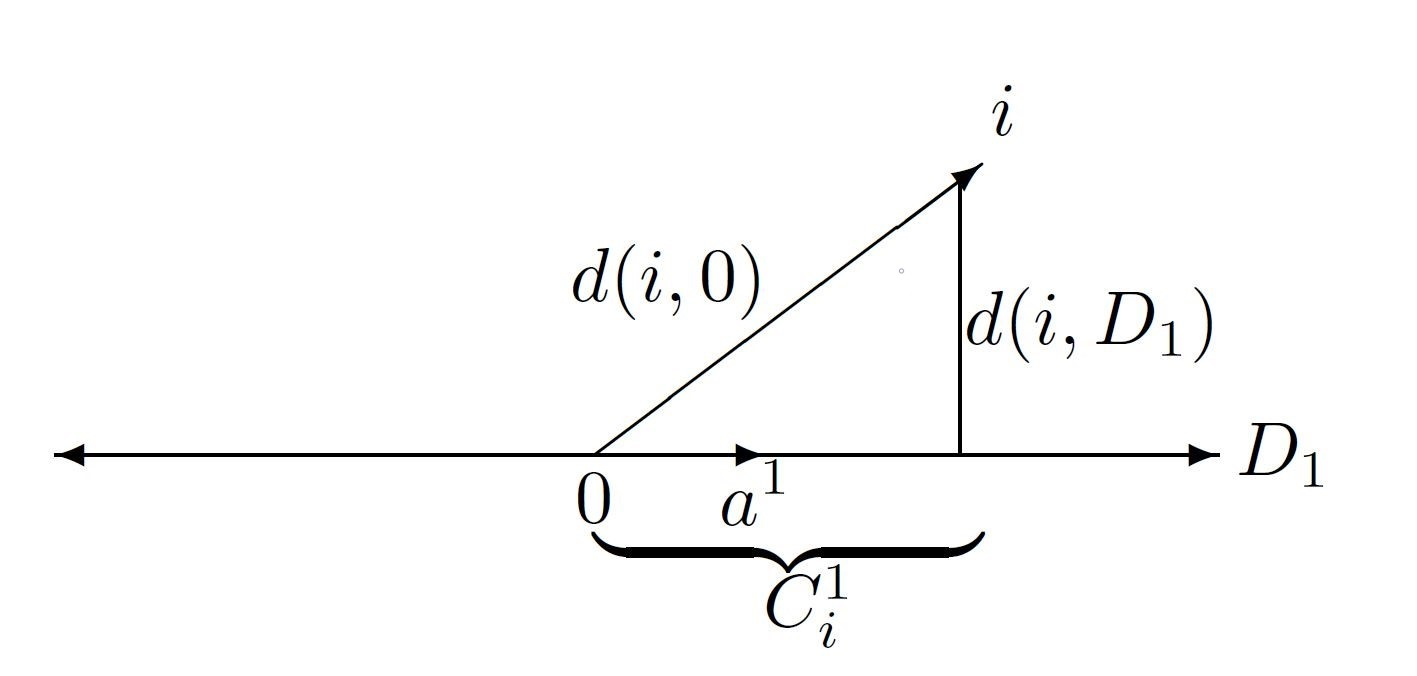
\includegraphics[width=0.7\textwidth]{figures/grafico.JPG}
        \label{graficoPitagoras}
\end{figure}
\begin{center}
    [Fuente:  Análisis de componentes principales]\cite{rojas2009analisis}
\end{center}

De la imagen \ref{graficoPitagoras} haciendo uso del teorema de 
Pitagoras se puede deducir $d^2(i,0)=(C_{i}^{1})^2+d^2(i,D_1)$, por lo que sumando sobre $i$ a ambos lados y multiplicando por $1/n$ se tiene que:

$$\dfrac{1}{n} \sum_{i=1}^{n}d^2(i,0)=\dfrac{1}{n}\sum_{i=1}^{n}(C_{i}^{1})^2+\dfrac{1}{n} \sum_{i=1}^{n}d^2(i,D_1)$$

Como $\dfrac{1}{n} \sum_{i=1}^{n}d^2(i,0)$ es independiente del eje $D_1$ que se escoja, se deduce que es una cantidad constante. por Lo tanto maximizar $\dfrac{1}{n}\sum_{i=1}^{n}(C_{i}^{1})^2$ termina siendo equivalente a minimizar $\dfrac{1}{n} \sum_{i=1}^{n}d^2(i,D_1)$

Siendo evidente que:

$$\dfrac{1}{n}\sum_{i=1}^{n}(C_{i}^{1})^2=\dfrac{1}{n}(C^1)^tC^1=\dfrac{1}{n}(a^1)^tX^tXa^1$$

Asi de esta manera el problema a resolver es:

\[\left\{ \begin{array}{rcl}
\mbox{max } \dfrac{1}{n} (a^1)^tX^tXa^1 \\
& & \\
\mbox{sujeto a } (a^1)^ta^1 \\
\end{array}
\right. \]

De manera que aplicando la proposición anterior con $B=\dfrac{1}{n}X^tX$ y $A=I_{mxm}$ se tiene que $a^1$ ser el vector propio del la norma 1 de la matriz $B=\dfrac{1}{n}X^tX$ asociado así al valor propio más grande.

\subsection{Teorema 2}

En la segunda etapa del PCA se calcula el eje de $D_2$ que pasa por el origen para el cual la dispersión de datos sea máxima, este eje $D_2$ pasa lo más cerca del conjunto de datos posible, queriendo decir así que el promedio de las distancias al cuadrado de los $n$ puntos del conjunto y el eje $D_2$ es minimal.

Siendo así $a^2$ el vector director de norma 1 en el eje $D_2$ el cual será ortogonal al vector $a^1$ construido en la etapa inicial, en este caso se tiene el siguiente problema de optimización:


\[\left\{ \begin{array}{rcl}
\mbox{max  } \dfrac{1}{n} (a^2)^tX^tXa^2 \\
& & \\
\mbox{sujeto}\left\{ \begin{array}{rcl}
(a^2)^ta^2=1 \\
& & \\
(a^2)^ta^2=0 \\
\end{array}
\right.  \\
\end{array}
\right. \]

Donde la solución viene a ser el vector propio asociado al segundo valor más grande de la matriz $V$ de varianzas-covarianzas.


\subsection{Teorema 3}

Para una etapa $k$ del PCA se calcula el eje de $D_k$ que pasa por el origen para la cual la dispersión del conjunto de datos sea máxima, así este eje $D_k$ pasa lo más cerca posible por el conjunto de datos, en otras palabras el promedio de las distancias al cuadrado de los $n$ puntos de la nube y el
eje $D_k$ es minimal.

Siendo $a^k$ el vector director del eje $D_k$ el cual será ortogonal al vector $A^r \forall r < k$ construidos en las etapas $1,2,...,k-1$, cuyo problema de optimización en este caso seria:

\[\left\{ \begin{array}{rcl}
\mbox{max  } \dfrac{1}{n} (a^k)^tX^tXa^k \\
& & \\
\mbox{sujeto}\left\{ \begin{array}{rcl}
(a^k)^ta^k=1 \\
& & \\
(a^k)^ta^k=0 \mbox{ para } r=1,2,...,k-1\\
\end{array}
\right.  \\
\end{array}
\right. \]

Donde la solución es el vector propio asociado al k-ésimo valor propio grande de la matriz de $V $ de varianzas-covarianzas que tenemos.

\section{Enfoque estadístico}
 \label{Enfoque estadístico}
  
Según las palabras del escritor Castillo Gonzalez se puede representar puntos p dimensionales con la mínima pérdida de información en un espacio de dimensión equivale a sustituir las p variables originales por una nueva variable, que resuma óptimamente la información. Esto significa que esta nueva variable debe tener la máxima relación con las originales, ees u decir, utilizar la variable de máxima variabilidad. \cite{CastilloGonzalez} 
  
El problema se reduce a encontrar una nueva dirección definida por
un vector unitario. Estadísticamente esto equivale a encontrar una segunda variable z2, encorralada con la anterior, y que tenga varianza
máxima.  
  
\section{Representación gráfica}
 Uno de los mayores usos que se obtienen de las representaciones gráficas, nos lo menciona el autor Castillo Gonzales "Las componentes principales permiten hacer una representación en pocas dimensiones de los hechos más sobresalientes de una tabla de datos." \cite{CastilloGonzalez}
 
 Hay 2 ejemplos representaciones gráficas, las cuales son:
 
 \subsection{Planos principales}
 Aquí se pueden apreciar las principales agrupaciones y dispersiones del individuo.
 
 Las coordenadas de un individuo sobre un plano principal se obtienen por la proyección del individuo sobre ese plano. Entonces un individuo \textit{i} se coloca en el plano principal por las coordenadas $(c_{\textit{i}}^{1},c_{\textit{i}}^{2})$ donde $c_{\textit{i}}^{1} = x_{\textit{i}}^{t}u_{1}$ y $c_{\textit{i}}^{1} = x_{\textit{i}}^{t}u_{2}$ (donde el vector $x_{\textit{i}}$ está centrado y estandarizado para cada variable.) 
 
 \textbf{Ejemplo 5} En el ejemplo de las notas escolares, el primer plano principal está generado por $c^{1}$ y $c^{2}$ dados en la Tabla 3.3. El plano principal es dado en la Figura 3.2. En la tabla 3.3 se puede ver que las coordenadas de Pedro son /0.67 y 1.64, y las de Sonia son 3.04 y 1.25, que son los valores usados para representarlos en el plano principal.
 
 \begin{figure}[H]
        \centering
        \caption{Primer plano principal para la tabla de notas escolares}
        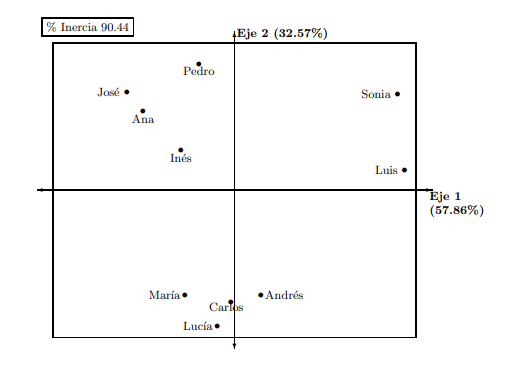
\includegraphics[width=0.8\textwidth]{figures/plano.png}
        \label{ejemplo5}
\end{figure}
\begin{center}
    [Fuente:  Análisis Multivariado de Datos, Métodos y Aplicaciones]\cite{CastilloGonzalez}
\end{center}

 
 \subsection{Círculos de correlaciones}
 Aquí se pueden apreciar las agrupaciones de variables y su comportamiento respecto de las componentes principales.  
 
 Los círculos de correlaciones se obtiene calculando el coeficiente de correlación lineal entre cada $x^\textit{j}$ en $c^{k}$. Por lo tanto:
\begin{center}
    
    Coordenada de la variable $x^\textit{j}$ en $ c^{k}: r(x^\textit{j},c^{k})$
    
\end{center} 
 
\textbf{Ejemplo 6} En la tabla de notas escolares, las correlaciones entre las variables originales y las dos primeros componentes principales son:

 \begin{figure}[H]
        \centering
        \caption{Siguiendo el procedimiento descrito anteriormente}
        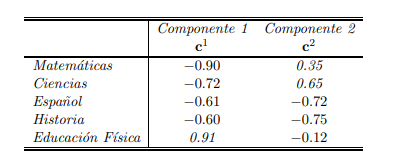
\includegraphics[width=0.8\textwidth]{figures/circulo.png}
        \label{ejemplo6}
\end{figure}
\begin{center}
    [Fuente:  Análisis Multivariado de Datos, Métodos y Aplicaciones]\cite{CastilloGonzalez}
\end{center}

 
 Por último, las dos gráficas anteriores son complementarias. Se puede apreciar el círculo de correlaciones permite interpretar las posiciones relativas de los individuos.
 Así mismo, se debe tener presente que estos no son más que simplificaciones de los hechos observados.
 
 
 \section{Interpretación de los resultados}
 

Como lo explica Joaquín\cite{interpretacion},
Una forma intuitiva de entender el proceso de PCA consiste en interpretar las componentes principales desde un punto de vista geométrico. Supóngase un conjunto de observaciones para las que se dispone de dos variables (X1, X2). El vector que define la primera componente principal (Z1) sigue la dirección en la que las observaciones varían más (linea roja). La proyección de cada observación sobre esa dirección equivale al valor de la primera componente para dicha observación. 

Como se puede observar en la siguiente imagen,

 \begin{figure}[H]
        \centering
        \caption{Siguiendo el procedimiento descrito, se pueden apreciar más datos}
        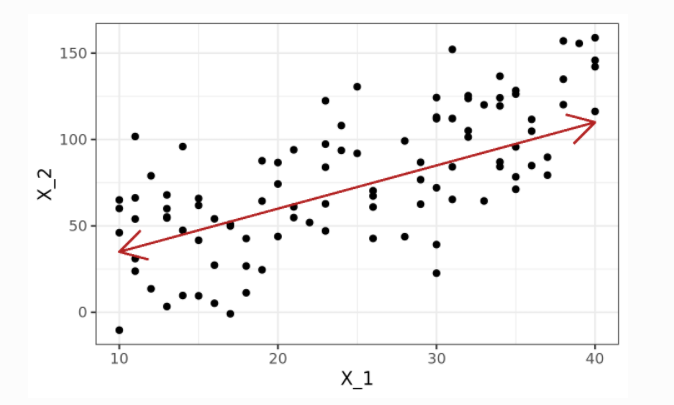
\includegraphics[width=0.8\textwidth]{figures/interpretacionDatos.PNG}
        \label{ilustracion vector Z1 }
\end{figure}
\begin{center}
    [Fuente:  Análisis Multivariado de Datos, Métodos y Aplicaciones]\cite{interpretacion}
\end{center}

La segunda componente $(Z2)$ sigue la segunda dirección en la que los datos muestran mayor varianza y que no está correlacionada con la primera componente. La condición de no correlación entre componentes principales equivale a decir que sus direcciones son perpendiculares.


 \begin{figure}[H]
        \centering
        \caption{Trayectoria de la segunda componente}
        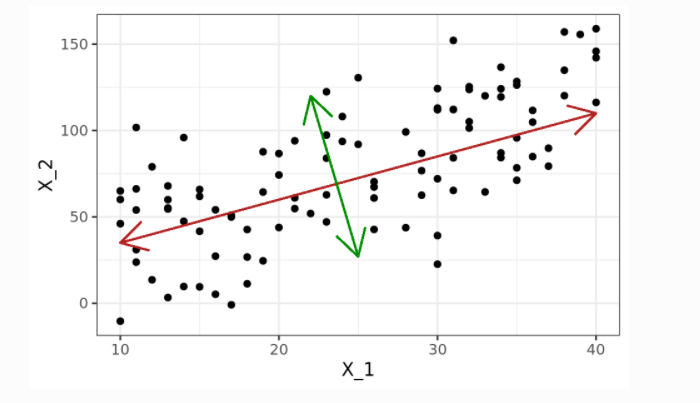
\includegraphics[width=0.8\textwidth]{figures/interpretacionDatos2.PNG}
        \label{ilustracion vector Z2 }
\end{figure}
\begin{center}
    [Fuente:  Análisis Multivariado de Datos, Métodos y Aplicaciones]\cite{interpretacion}
\end{center}


 Para la interpretación de componentes, se debe de tener en cuenta la subjetividad del sujeto. 
 Es el asunto más importante de un Análisis de Componentes Principales es la interpretación de los resultados. A pesar de que, como en toda técnica estadística, en la interpretación hay mucho de arte y la experiencia juega un papel importante, se pueden sugerir algunas directrices que pueden ayudar a encontrar los hechos más sobresalientes en los resultados.

En primer lugar, se debe tratar de etiquetar a las componentes principales. Para ello, se usarán las medidas de calidad de representación de los individuos y de las variables. \cite{CastilloGonzalez}
 
